
% !TEX encoding = UTF-8 Unicode

\documentclass[a4paper]{article}

\usepackage{color}
\usepackage{url}
\usepackage[T2A]{fontenc}
\usepackage[utf8]{inputenc}
\usepackage{graphicx}

\usepackage[english,serbian]{babel}

\usepackage[unicode]{hyperref}
\hypersetup{colorlinks,citecolor=green,filecolor=green,linkcolor=blue,urlcolor=blue}

\begin{document}
	\title{Proširena stvarnost i mogućnosti njene upotrebe u obrazovanju\\ \vskip 0.2in \small{Seminarski rad u oviru kursa\\ Tehničko i naučno pisanje\\ Matematički Fakultet}}
	
	\author{Autori: \\ Filip Nedeljković\\ Matija Đorđević\\ Mlađan Simić\\ Igor Stojanović}
	\date{11.~novembar 2022.}
	\maketitle
	
	\abstract{
		Proširena stvarnost je tehnologija koja se počela koristiti početkom 90-ih godina prošlog veka, tada u vojnoj instituciji vazdušnih snaga SAD-a. 
		Sam termin „proširena stvarnost“ skovan je 1990. godine. Samim time, radi se o relativno novoj tehnologiji. U radu je prikazan njen razvoj, 
		razvoj hardvera i softvera koji je ključan za rad, širu dostupnost i mogućnosti proširene stvarnosti, kako je tehnologija postala šire dostupna, 
		način na koji se ova tehnologija može iskoristiti na šta ćemo fokus staviti na primenu tehnologije proširene stvarnosti u obrazovanju.
	}
	
	\tableofcontents
	
	\newpage
	
	\section{Uvod}
	\label{sec:Uvod}
	Proširena stvarnost (engl. Augmented reality, skraćeno AR) predstavlja takav spoj fizičkog i digitalnog sveta, u kojem digitalni elementi (slika, tekst, 
	animacija ili zvuk) dopunjavaju fizički svet. Ljudi traže prirodniji, efikasniji i pristupačniji način za interakciju sa računarima i današnjim digitalnim 
	svetom. Iz tog razloga okreće se tehnologijama AR i VR (engl. Virtual reality - virtuelna stvarnost). Glavna razlika između ovih tehnologija je u tome što VR 
	zamenjuje predstavljanje stvarnog sveta, dok AR dodaje informacije stvarnom svetu, zbog čega postoji i razlika u korišćenom hardveru. Međutim, VR i AR 
	tehnologije ne isključuju jedna drugu, naprotiv, često su komplementarne jedna drugoj, a razvoj i primena jedne je uticala na razvoj i primenu druge. AR 
	tehnologija nam omogućava da vidimo elemente koji ne postoje u stvarnom životu putem aplikacije kroz ekran uređaja, obično mobilnog telefona.Tehnologija 
	proširene stvarnosti (AR) se koristi u mnogim oblastima kao što su zabava, vojska, marketing, inženjering, medicina, psihologija, oglašavanje. S obzirom na 
	naprednu tehnologiju i bogato okruženje za učenje koje nudi AR, istaknuta je i primena ove tehnologije u oblasti obrazovanja. Za razliku od AR, VR tehnologija 
	zahteva upotrebu naočara kroz koje ne možete videti ništa oko sebe, već samo virtuelno stvoreni svet. Obe tehnologije su veoma mlade, njihov razvoj počinje u 
	drugoj polovini 20. a šira upotreba i dostupnost tek početkom 21. veka. Ali, uprkos tome, sve brži tehnološki napredak i globalizacija doveli su do toga da se 
	obe tehnologije veoma brzo šire, postaju dostupne sve većem broju ljudi, a svakim danom im se pronalaze nove potencijalne upotrebe.

	\section{Istorija}
    \label{sec:Istorija}
    Od početka civilizacije, ljudi su težili unapređenju svog okruženja. Rani pokušaji obuhvatali su manipulaciju objekata u fizičkom smislu a kako se čovečanstvo razvijalo, ideje su dobile vodeći značaj. Uz pomoć novih uređaja i pomagala, ulazi se u vreme u kome nestaju granice između fizičkog i idejnog sveta.\\
    Pojam „proširene realnosti“ je tek u skorije vreme postao popularan, ali su se ljudi ovom tematikom bavili stotinama godina koristeći se optičkom naukom. Još u 17. veku poznat je primer „Peperovog duha“, pozorišna iluzionistička tehnika koja je reflekcijom posmatraču dala utisak viđenja duha. U toku Drugog svetskog rata, Vojska Velike Britanije razvila je tehnologiju koja je omogućila prikaz radarskih informacija na vetrobranu borbenih aviona i time olakšao prepoznavanje neprijatelja.\\
    Kinematograf Morton Hejlig je u periodu od 1955. do 1962. godine radio na projektu zvanom „Sensorama“ koji je, njegovim rečima, predstavljao „budućnost filma i bioskopa“ jer je umesto statičnog posmatranja, nudio bliži osećaj prisutnosti.\\
    Ubrzanim razvojem računarskih nauka i arhitekture računara otvorilo se novo poglavlje proširene realnosti. Ajvan Saderland je razvio Sketchpad, prvu interaktivnu grafičkuaplikaciju na Masačusetskom Institutu Tehnologije 1963. godine.\\
    Pet godina kasnije, na Harvard Univerzitetu, zajedno sa Bobom Sprulom, stvara prvi prototip sistema proširene realnosti kakve je danas znamo. Prototip se sadržao od displeja postavljenog preko cele glave korisnika sa brojnim kablovima povezanim na velike kompjutere. Iako primitivan, sistem je omogućavao prikaz trodimenzionalne grafike prikazane preko stvarnosti. Korisnik je imao 40 stepeni vidnog polja, a posrebrena ogledala u prizmi su zaslužne za prikaz slike iz katodne cevi i realnosti istovremeno.\\
    Majron Kruger je 1975. godine uspostavio laboratoriju za veštačku realnost na Univerzitetu u Konektikutu zvanu „Videoplace“. Njegova ideja se zasnivala na proširenoj realnosti koja nije podrazumevala korišćenje pomagala poput naočara ili rukavica. „Videoplace“ je koristio projektore, kamere, specijalizovani hardver i siluete korisnika kako bi prilagodio virtuelno okruženje. Pokreti korisnika su analizirani i obrađeni tako da se promene vide u realnom vremenu.\\
    Na vrhuncu Hladnog rata, najveći budžet za projekte ove tematike dodeljivan je, očekivano, onima sa vojno-industrijskom svrhom. Uglavnom se radilo na unapređenju kokpita vojnih aviona a značajni pomaci ostvarivani su u Amrstrong Laboratoriji (Američko ratno vazduhoplovstvo), Ames Istraživačkom centru (NASA), Univerzitetu Severne Karoline, i tako dalje. Interesantan primer je tenkovski simulator koji je napravila vojska Švajcarske. Imao je za cilj osposobljavanje korisnika da upravljaju tenkom bez potrebe da ih stavi u potencijalno opasnu situaciju gde je svaka greška poprilično skupa.\\
    Devedesetih godina prošlog veka, proširena realnost dobija svoju formalnu definiciju, i to u naučnom radu Ronalda Azume koji je identifikuje kao spoj stvarnog i virtuelnog okruženja gde su oba interaktivna u realnom vremenu. Sistemi se koriste za razne nove funkcionalnosti poput navigacije, medicine, edukacije, itd.\\
    Prva igrica u proširenoj realnosti je ARQuake, razvijena od strane Brusa Tomasa 2000. godine i predstavljena na Internacionalnom simpozijumu prenosnih računara. Hirokazu Kato u periodu dvehiljaditih razvija open-source biblioteku nazvanu „ArToolKit“ koja pomaže ostalim programerima pri razvoju aplikacija u proširenoj realnosti.\\ 
    U nastavku prve decenije, Microsoft je razvio „Kinect“, uređaj za detekciju pokreta i odvajanje korisnika od okoline, primarno korišćen za razonodu. Funkcioniše na strukturisanim svetlosnim računanjima, koja se izvode uz RGB kamere i infracrvene projektore i detektore.\\
    Google Glass je razvijen od strane Google X, ustanove u okviru Google-a posvećenoj tehnološkim dostignućima. Manji je i tanji nego bilo koji prethodni pokušaj dizajna prenosivih naočara. Liči na standardne naočare, sa sočivima zamenjenim monitorom. Glass je predstavljao inovativan koncept ali nije uspeo da se probije na tržištu.\\
    Razvoj mobilnih uređaja koji sada poseduju sredstvo za navigaciju, fotografisanje, reprodukciju zvuka i snimka, žiroskope, itd., omogućio je nastanak mnoštva aplikacija koje su kombinovale sve te aspekte i zapravo stvorile jedno okruženje proširene realnosti. Najpopularniji primer je igrica Pokemon GO koja je za kratko vreme osvojila svet.\\ 
    Potencijal koji se nalazi u ovoj tehnologiji je velik i nesumnjivo je da će u jednom trenutku biti uveliko prihvaćena od strane šire javnosti i prosečnih ljudi za njihove različite potrebe.
	
	\section{Primena}
	\label{sec:Primena}
	Obrazovni sistem evoluira i prilagođava se dostupnoj tehnologiji i potrebama studenata. Tradicionalne knjige zamenjuju se digitalnim nastavnim sadržajima. 
	U većini akademskih oblasti, kao što su \emph{matematika, nauka, inženjerstvo i statistika}, uspeh u ime studenta u velikoj meri zavisi od njegove sposobnosti da 
	predvidi i manipuliše apstraktnim informacijama. Jedan od glavnih razloga zašto se VR i AR koriste u svrhe obrazovanja i obuke je podrška visoke interaktivnosti 
	i sposobnosti predstavljanja virtuelnog okruženja koje podseća na stvarni svet. Pomoću ove tehnologije moguće je istraživanje i manipulisanje trodimenzionalnim 
	interaktivnim okruženjem. Tradicionalne metode obrazovanja zasnovane na predavanjima suočavaju se sa problemom nedovoljne  angažovanosti studenata, što za posledicu 
	može da ima negativan uticaj na njihov uspeh.


	Istraživači potvrđuju da tehnološki alati koji se koriste u obrazovanju doprinose aktiviranju motivacije, nude nove mogućnosti, pružaju prijatnu atmosferu za učenje, 
	povećavaju interakciju među učenicima, čine proces učenja aktivnijim, efikasnijim i sadržajnijim. Na sličan način AR tehnologija privlači pažnju naučnika u obrazovanju 
	jer favorizuje interakciju stvarnih i virtuelnih objekata i stvara okruženje koje podstiče iskustveno učenje. Naučnici smatraju da AR tehnologija pomaže u predstavljanju 
	apstraktnih stvari, u prikazivanju opasnih slučajeva, prikazivanju složenih tema, zatim u podučavanju nevidljivih stvari i događaja. Štaviše, AR tehnologija pruža studentima 
	fleksibilnost, podstiče veštine kreativnog razmišljanja, veštine tumačenja i rešavanja problema. Mnogi naučnici koji istražuju upotrebu tehnologije i interneta u obrazovanju 
	ukazuju na značaj karakteristika učenika i upotrebe tehnologije za poboljšanje ishoda učenja u oblasti visokog obrazovanja.

	\emph{Construct3D} omogućava studentima da uče koncepte mašinstva, matematike ili geometrije. Nastavni sadržaji iz matematike koji se odnose na tri dimenzije mogu biti teški za učenike 
	jer moraju stalno u glavi da pretvaraju dvodimenzionalni crtež iz udžbenika u trodimenzionalni model i obrnuto. Zbog toga učenici imaju dodatni izazov u kome treba da steknu 
	trodimenzionalna znanja iz dvodimenzionalnih materijala. Trenutno se ovaj problem donekle rešava uz pomoć fizičkih modela geometrijskih tela i 3D grafičkih kalkulatora (npr. \emph{GeoGebra 3D kalkulator}).
	
	AR aplikacije za hemiju omogućavaju studentima da vizuelizuju i komuniciraju sa prostornom strukturom molekula koristeći ručni marker. \emph{HP Reveal}, besplatna aplikacija, koristi 
	se za kreiranje AR kartica za proučavanje mehanizama organske hemije i za kreiranje virtuelnih demonstracija kako se koriste laboratorijski instrumenti.

	Deca u osnovnoj školi lako uče iz interaktivnih iskustava. Astronomska sazvežđa \ref{fig:Primer korišćenja} 
	\begin{figure}[h!]
		\begin{center}
		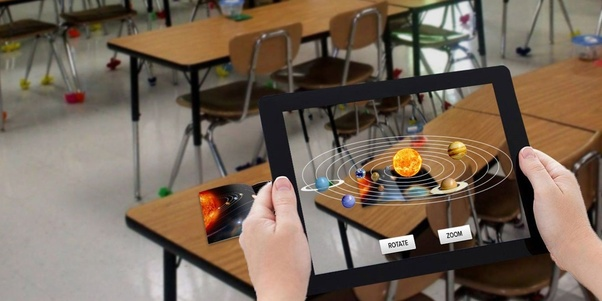
\includegraphics[scale=0.5]{primerkorišćenja.jpg}
		\end{center}
		\caption{Primer korišćenja}
		\label{fig:Primer korišćenja}
		\end{figure}
	i kretanje objekata u Sunčevom sistemu mogu se prikazati u pravcu u kome se uređaj drži
	i proširiti dodatnim video informacijama. Ilustracije naučnih knjiga na papiru mogu da zažive u vidu video zapisa bez potrebe da učenik traži video materijale na internetu.

	Proširena stvarnost se može koristiti i kao pomoćno sredstvo u radu sa učenicima koji imaju smetnje u razvoju. Jedan mogući okvir učenja koji koristi proširenu stvarnost 
	i gamifikaciju koja nudi dodatnu podršku učenicima sa intelektualnim teškoćama u procesu učenja je da učenici grupišu predmete koji pripadaju životinjama ili voću. 
	Učenici biraju oznake sa nazivima i postavljaju ih ispred kamera, nakon čega se na računaru kreira slika izabrane životinje/voća i računar izgovara naziv životinje/voća.


	\section{Zaključak}
	\label{sec:Zaključak}
	U okruženju koje ima karakteristike globalizovanog, dinamičnog i visoko \hyphenation{konku-re-tnog} konkuretnog, prihvatanje i implementacija digitalnih 
	tehnologija postaje neminovna. U takvim uslovima obrazovne institucije suočavaju se sa potrebom da uvrste iste u svoj rad. VR i AR se sve više primenjuje
	u okviru obrazovnih procesa i njihov potencijal umnogome doprinosi studentima. U radu je istaknuto nekoliko od brojnih prednosti koje tehnologija koja prevodi
	čoveka u virtuelni svet nosi sa sobom. Po ugledu na primer poznatih svetskih univerziteta i njihovo široko usvajanje virtuelne i proširene stvarnosti, prepoznat 
	je značaj praćenja trendova u obrazovnoj tehnologiji. Upotreba VR i AR tehnologije i efekti te upotrebe veoma su raznoliki, ali ono što se izdvaja kao zajedničko 
	jeste mogućnost neposredne interakcije sa fizički nedostupnim objektima i upoznavanje sa predmetima i situacijama na interesantan i razumljiv način.
	
        \addcontentsline{toc}{section}{Literatura}
        \iffalse
        \bibliography{seminarski} 
        \bibliographystyle{plain}
        \fi
        
        \begin{thebibliography}{9}
        \bibitem{Primena AR tehnologije obrazovanju 1} E. Solak i R. Cakir. Investigating the Role of Augmented Reality Technology in the Language Classroom. Amasija, 
	Turska, 2015.
        \bibitem{Proširena stvarnost} P. Pleše. Proširena stvarnost. Zagreb, Hrvatska, 2019.
        \bibitem{Upotreba AR tehologije u obrazovanju 2} K. Mitrović, J. Čurčić, A. Jakšić, B. Bogojević i D. Gračanin. Primena tehnologije virtuelne I proširene 
	stvarnosti u obrazovanju. Novi Sad, Srbija, 2020.
        \bibitem{Upotreba kod dece sa intelektualnim teškoćama} K. Stančin. Upotreba informacijsko-komunikacijske tehnologije u odgoju i obrazovanju učenika s 
	intelektualnim teškoćama, Zagreb, Hrvatska, 2018.
        \bibitem{Princip rada tehnologije proširene stvarnosti} A. B. Craig. Understanding Augmented Reality: Concepts and Applications. Ilinois, Sjedinjene Američke 
	Države, 2013.
 
        \end{thebibliography}

\end{document}
